\section{Visual Document Matching}
\label{sec:method_modeling}

Traditional classification methods, such as entropy learning, lock the generality of the model to the set of classes it has been trained on. Therefore, the use of Zero Shot Learning techniques is essential to be able to classify document layouts that have not been seen on the training set. \blue{Among the possible \gls{ZSL} solutions, we use metric learning with Siamese networks to achieve this goal. The proposed metric learning framework, \gls{VDM}, takes two different document images, and compares them to decide whether they belong to the same class or not, using vision models to match documents that share the same class.}

\blue{This approach is inspired by biometric signature verification approaches~\cite{jiang_dsdtw_2022}, where a system has a repository of ground-truth signature references (signatures that they know are from a certain person), and they compare them with a query signature, to verify if they belong to the same person or not. }Therefore, \gls{VDM} works by learning to draw representations of documents in a feature space with $n$ dimensions, such that documents that share the same class are represented as clustered together, and documents that have different classes are far apart, as illustrated in \refFig{fig:vector_space_mapping}.

\begin{figure*}[t!]
    \begin{subfigure}[b]{0.9\textwidth}
        \centering
        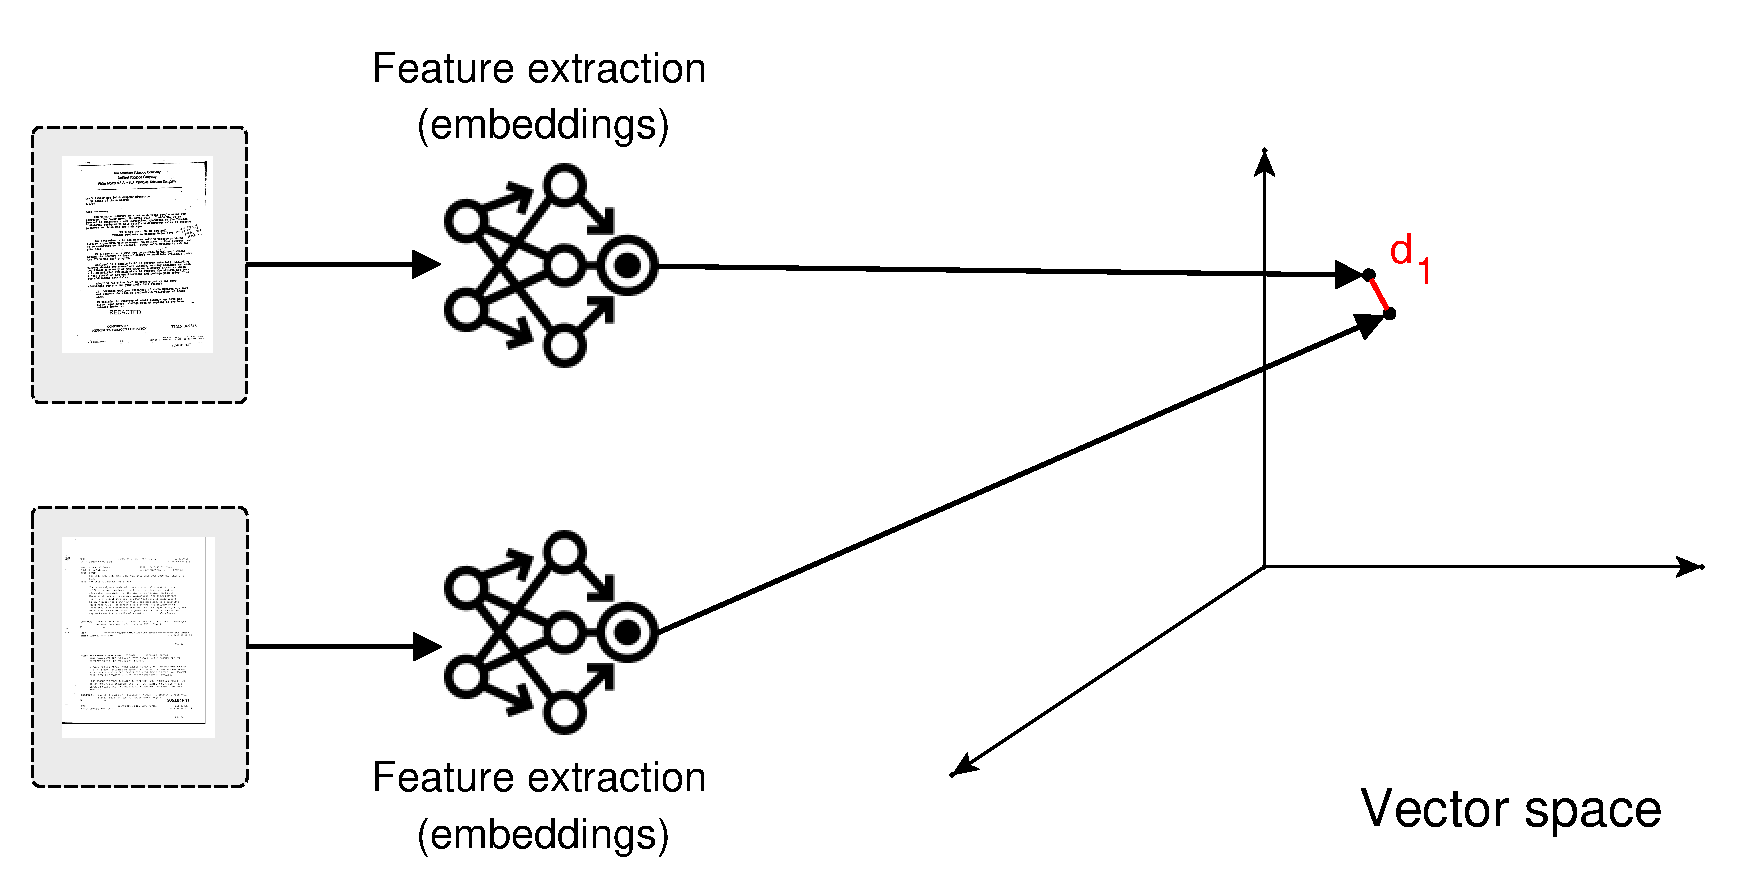
\includegraphics[width=\textwidth, trim=15 0 30 0, clip]{images/vector_space_1.pdf}
        \caption{Similar documents with small distance $d_1$ between them.}
        \label{fig:similar_docs}
    \end{subfigure}
    \vfill
    \begin{subfigure}[b]{0.9\textwidth}
        \centering
        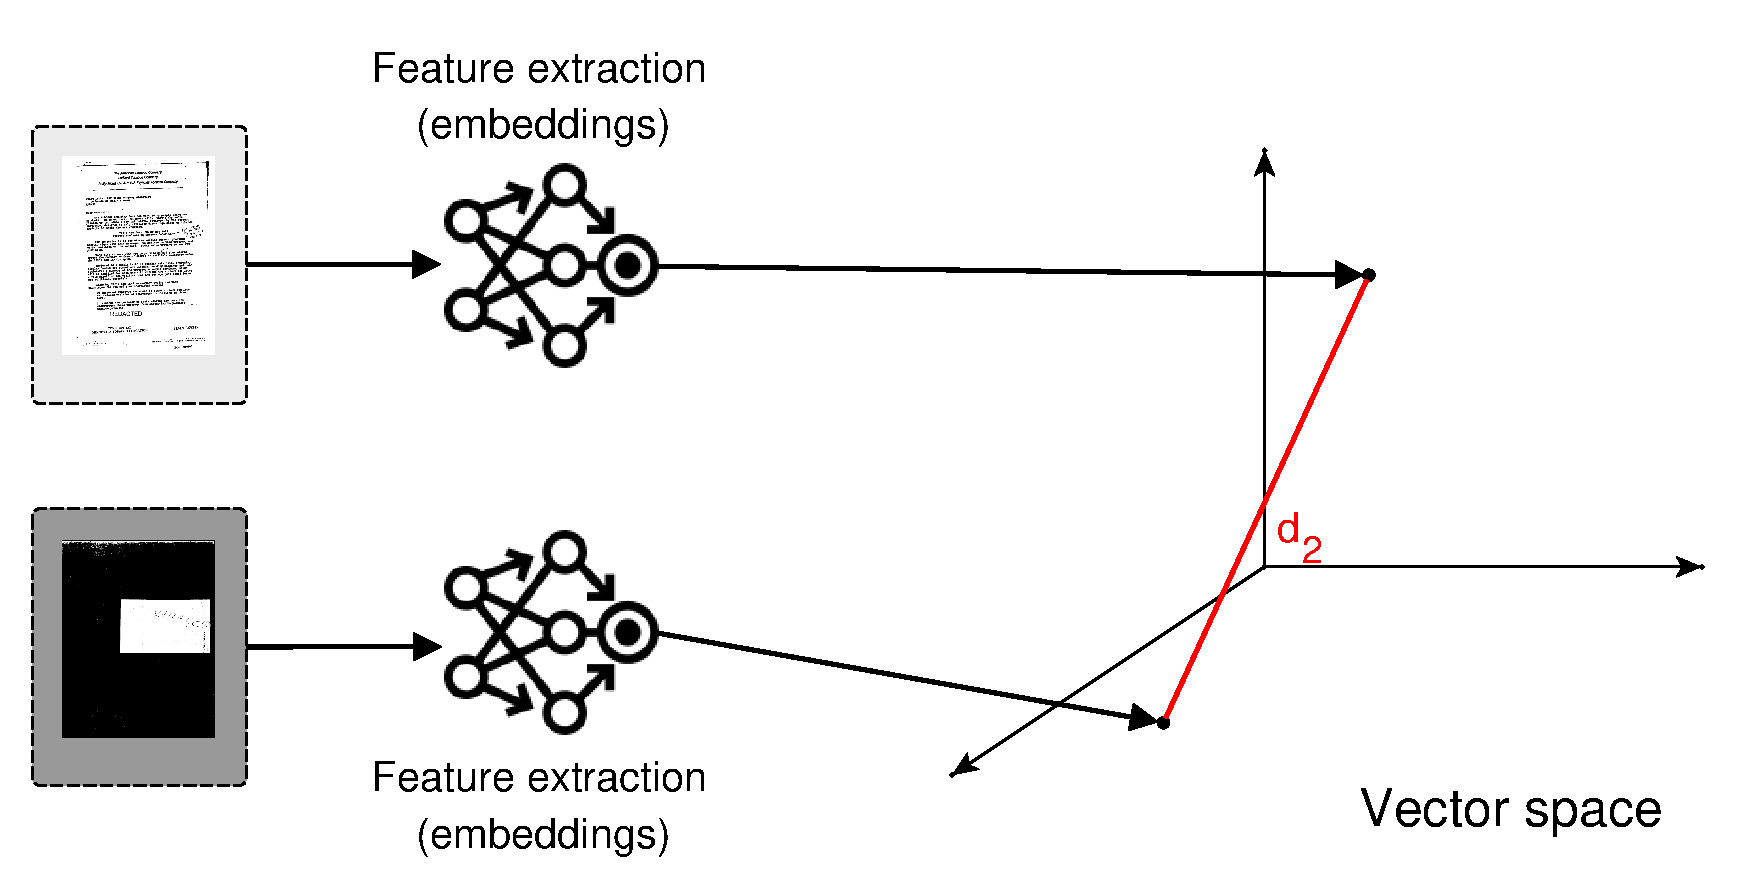
\includegraphics[width=\textwidth, trim=15 0 30 0, clip]{images/vector_space_2.pdf}
        \caption{Dissimilar documents with large distance $d_2$ between them.}
        \label{fig:dissimilar_docs}
    \end{subfigure}
    \caption{Illustration of two documents mapped to the vector space that are similar (a) and dissimilar (b). This document mapping to a vector space is performed by the proposed learned method for similarity analysis. Visually similar documents have a smaller distance in the projected space than dissimilar ones.}
    \label{fig:vector_space_mapping}
\end{figure*}

A wide variety of backbones are used to experiment on the proposed dataset, but they all follow the same metric learning architecture with Siamese Networks. They are AlexNet~\cite{krizhevsky_imagenet_2012}, VGG~\cite{simonyan_very_2015}, ResNet~\cite{he_deep_2016}, MobileNetV3~\cite{howard_searching_2019}, EfficientNet~\cite{tan_efficientnet_2019} and \gls{ViT}~\cite{dosovitskiy_image_2021}. To adapt the architectures to a Siamese network, only the last linear layer of each model --- the classification layer --- is modified into a new linear layer with an arbitrary size $n$, suitable for the problem.
